\documentclass{mcmthesis}
  \makeatletter
  \newcommand{\rmnum}[1]{\romannumeral #1}
  \newcommand{\Rmnum}[1]{\expandafter\@slowromancap\romannumeral #1@}
  \makeatother

\mcmsetup{CTeX = false,   % 使用 CTeX 套装时,设置为 true
        tcn = 91397, problem = C,
        sheet = true, titleinsheet = true, keywordsinsheet = true,
        titlepage = false, abstract = true}
\usepackage{palatino}
\usepackage{lipsum}
\usepackage{cite}
\usepackage{amsmath}  
\usepackage{amssymb}
\usepackage{url}
\usepackage{subfigure}
\usepackage{float}


\setlength{\parindent}{1.5em}

\title{}
\begin{document}
\begin{abstract}
abstract
\begin{keywords}
keyword1; keyword2
\end{keywords}
\end{abstract}
\maketitle


\tableofcontents
% \thispagestyle{}% 当前页不显示页码'
\pagestyle{fancy} 
\rhead{\small\sffamily  \rmnum{\thepage}}
\newpage
\pagestyle{fancy}
\rhead{\small\sffamily Page \thepage\ of \pageref{LastPage}}
\setcounter{page}{1}

\section{Introduction}

\section{Energy Profile}
\subsection{Overview}
\subsection{title}

\subsubsection{Arizona}
\begin{figure}[H]
\begin{minipage}[htb]{0.5\textwidth}
\centering
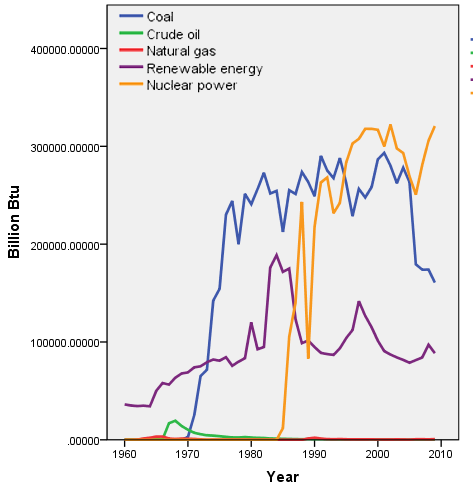
\includegraphics[width=3in]{AZPRB.png}
\caption{AZPRB} \label{fig:AZPRB}
\end{minipage}
\begin{minipage}[htb]{0.5\textwidth}
\centering
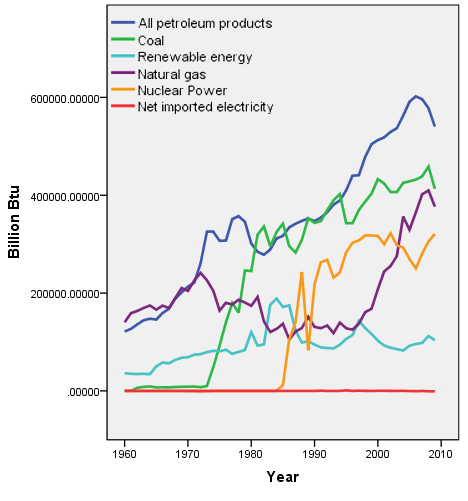
\includegraphics[width=3in]{AZTCB.png}
\caption{AZTCB} \label{fig:AZTCB}
\end{minipage}
\end{figure}

\begin{figure}[H]
\begin{minipage}[htb]{0.5\textwidth}
\centering
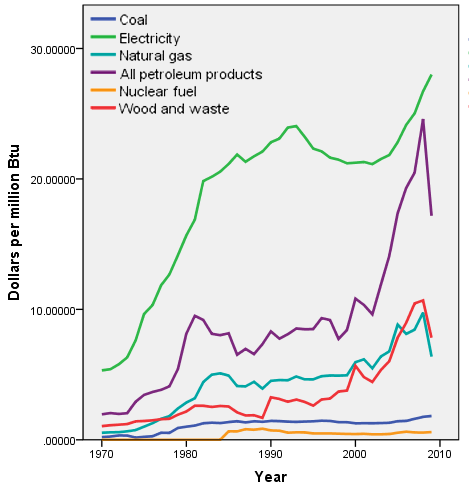
\includegraphics[width=3in]{AZTCD.png}
\caption{AZTCD} \label{fig:AZTCD}
\end{minipage}
\begin{minipage}[htb]{0.5\textwidth}
\centering
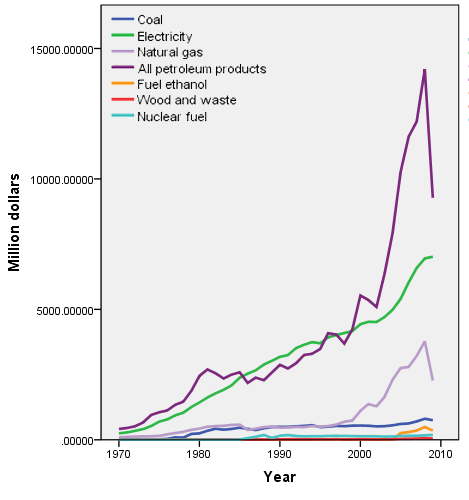
\includegraphics[width=3in]{AZTCV.png}
\caption{AZTCV} \label{fig:AZTCV}
\end{minipage}
\end{figure}

\subsubsection{California}
\begin{figure}[H]
\begin{minipage}[htb]{0.5\textwidth}
\centering
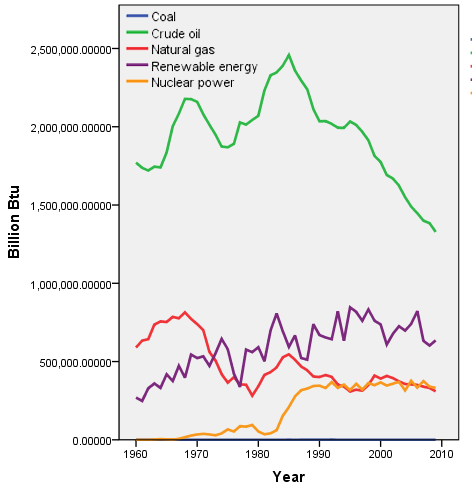
\includegraphics[width=3in]{CAPRB.png}
\caption{CAPRB} \label{fig:CAPRB}
\end{minipage}
\begin{minipage}[htb]{0.5\textwidth}
\centering
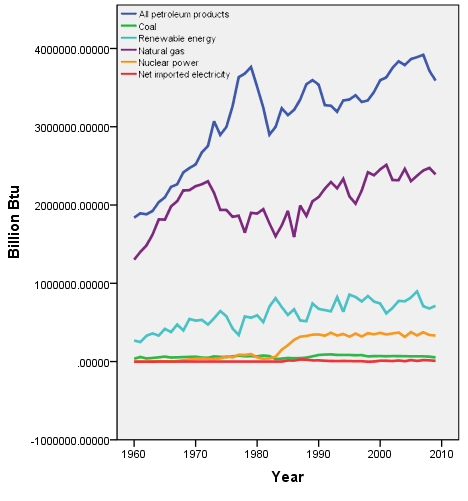
\includegraphics[width=3in]{CATCB.png}
\caption{CATCB} \label{fig:CATCB}
\end{minipage}
\end{figure}

\begin{figure}[H]
\begin{minipage}[htb]{0.5\textwidth}
\centering
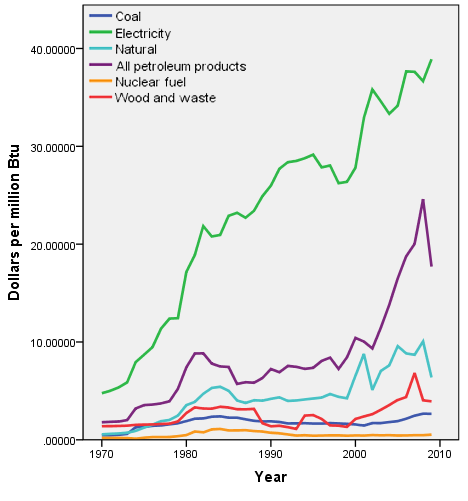
\includegraphics[width=3in]{CATCD.png}
\caption{CATCD} \label{fig:CATCD}
\end{minipage}
\begin{minipage}[htb]{0.5\textwidth}
\centering
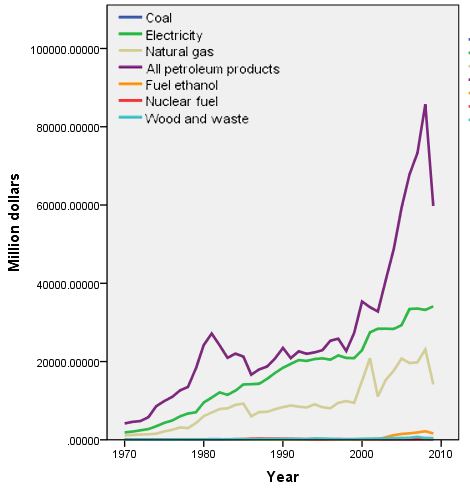
\includegraphics[width=3in]{CATCV.png}
\caption{CATCV} \label{fig:CATCV}
\end{minipage}
\end{figure}

\subsubsection{New Mexico}
\begin{figure}[H]
\begin{minipage}[htb]{0.5\textwidth}
\centering
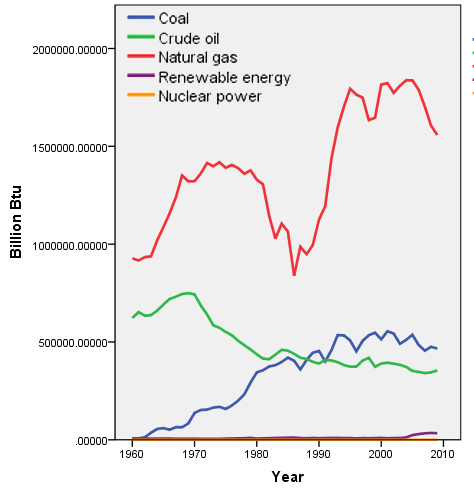
\includegraphics[width=3in]{NMPRB.png}
\caption{NMPRB} \label{fig:NMPRB}
\end{minipage}
\begin{minipage}[htb]{0.5\textwidth}
\centering
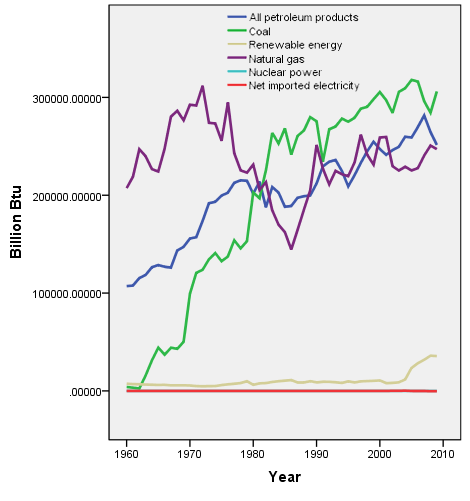
\includegraphics[width=3in]{NMTCB.png}
\caption{NMTCB} \label{fig:NMTCB}
\end{minipage}
\end{figure}

\begin{figure}[H]
\begin{minipage}[htb]{0.5\textwidth}
\centering
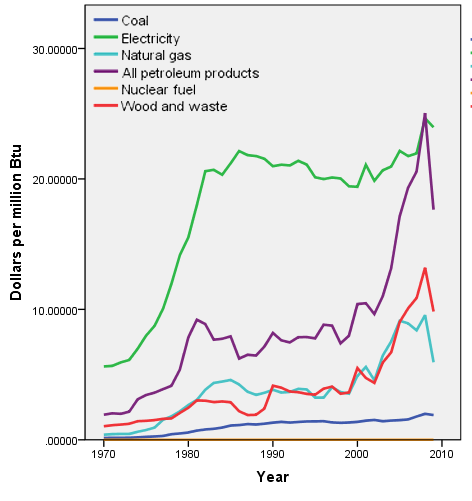
\includegraphics[width=3.in]{NMTCD.png}
\caption{NMTCD} \label{fig:NMTCD}
\end{minipage}
\begin{minipage}[htb]{0.5\textwidth}
\centering
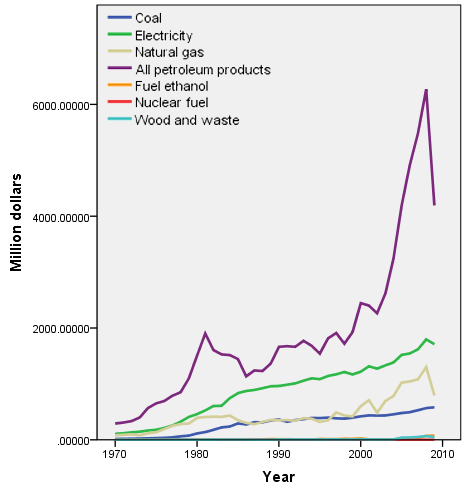
\includegraphics[width=3in]{NMTCV.png}
\caption{NMTCV} \label{fig:NMTCV}
\end{minipage}
\end{figure}

\subsubsection{Texas}
\begin{figure}[H]
\begin{minipage}[htb]{0.5\textwidth}
\centering
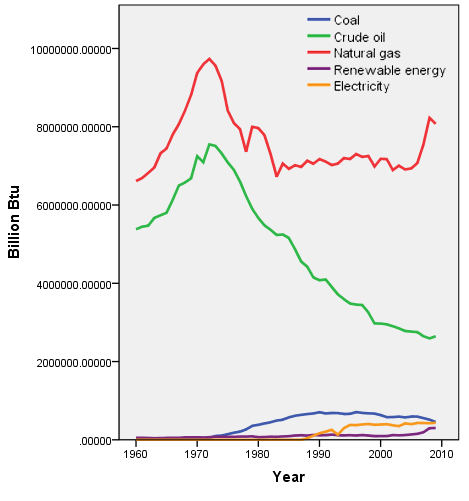
\includegraphics[width=3in]{TXPRB.png}
\caption{TXPRB} \label{fig:TXPRB}
\end{minipage}
\begin{minipage}[htb]{0.5\textwidth}
\centering
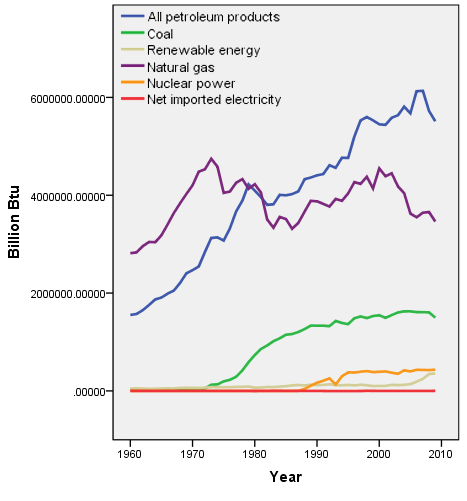
\includegraphics[width=3in]{TXTCB.png}
\caption{TXTCB} \label{fig:TXTCB}
\end{minipage}
\end{figure}

\begin{figure}[H]
\begin{minipage}[htb]{0.5\textwidth}
\centering
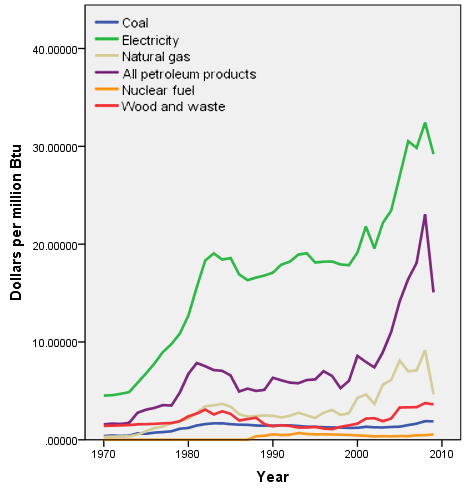
\includegraphics[width=3in]{TXTCD.png}
\caption{TXTCD} \label{fig:TXTCD}
\end{minipage}
\begin{minipage}[htb]{0.5\textwidth}
\centering
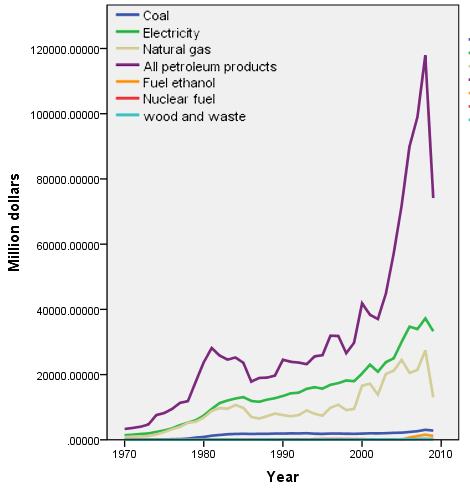
\includegraphics[width=3in]{TXTCV.png}
\caption{TXTCV} \label{fig:TXTCV}
\end{minipage}
\end{figure}






\newpage
\setcounter{page}{2}
\pagestyle{fancy} 
\rhead{\small\sffamily  \rmnum{\thepage}}

% \cite{PEISHI1989297}

% \cite{timmurphy.org}

% \bibliographystyle{siam}
% \bibliography{test}



\begin{appendices}

\begin{proof}   %插入证明
  x
\end{proof}

\newtheorem{lemma}{Lemma}%只需在第一个引理开始之前出现一次  
\begin{lemma}  
If $f\in C_{L}^{1,1}(\mathbb{R}^{n})$, then $\forall \textbf{x},\textbf{y}\in\mathbb{R}^{n}$ we have  
\begin{equation}  
\left|{f(\textbf{y})-f(\textbf{x})-\nabla f(\textbf{x})^{T}(\textbf{y}-\textbf{x})}\right|\le\frac{L}{2}\left\|{\textbf{y}-\textbf{x}}\right\|^{2}.  
%\label{eq:eq5}  
\end{equation}  
%\label{lem:lem1}  
\end{lemma} 
\section{First appendix}

\lipsum[13]

% 代码插入
Here are simulation programmes we used in our model as follow.\\

\textbf{\textcolor[rgb]{0.98,0.00,0.00}{Input matlab source:}}
\lstinputlisting[language=Matlab]{./code/mcmthesis-matlab1.m}

\section{Second appendix}

some more text \textcolor[rgb]{0.98,0.00,0.00}{\textbf{Input C++ source:}}
\lstinputlisting[language=C++]{./code/mcmthesis-sudoku.cpp}

\end{appendices}
\end{document}

